\documentclass[11pt,a4paper]{article}

% ---------- Encoding and typography ----------
\usepackage[T1]{fontenc}
\usepackage[utf8]{inputenc}
\usepackage{lmodern}
\usepackage{microtype}

% ---------- Page layout ----------
\usepackage[a4paper,margin=1in]{geometry}
\usepackage{setspace}
\setstretch{1.15}

% ---------- Math, figures, tables ----------
\usepackage{amsmath,amssymb}
\usepackage{graphicx}
\usepackage{booktabs}
\usepackage{siunitx}

% ---------- References and links ----------
\usepackage[numbers,sort&compress]{natbib}
\usepackage[hidelinks]{hyperref}
\usepackage[nameinlink,noabbrev]{cleveref}

% ---------- Header/footer ----------
\usepackage{fancyhdr}
\pagestyle{fancy}
\fancyhf{}
\setlength{\headheight}{14pt}
\lhead{Simplex Work Test}
\rhead{\thepage}

% ---------- Title metadata ----------
\title{Belief State Geometries for Non-Ergodic Data-Generating Processes}
\author{Aden Power\thanks{LLMs used extensively for coding and data processing, but not for prose.} \\ Simplex Work Test}
\date{\today}

\begin{document}

\maketitle
\thispagestyle{fancy}

\begin{abstract}
In this work test:
\begin{itemize}
\item I describe in theory the hypothetical belief state geometries for a non ergodic process generated by multiple Mess3's,
\item I follow the Simplex approach to empirically test this and find representations of one of the candidate geometries in the residual stream,
\item I describe a change in coordinates of the simplex geometry that more closely corresponds with the representations from the model,
\item I give evidence to show that different Mess3 processes are similar enough that the transformer effectively learns to represent their states together in a small number of dimensions in superposition,
\item I describe and implement a method to steer the model towards predicting one of the processes over the others, but fail to verify its accuracy.
\end{itemize}
\end{abstract}

\section{Introduction}
Transformers have been shown to contain linearaly transformed representations of the belief state geometry in their residual streams. Real data-generating processes can often be at least approximately factored. For example, consider some data obtained from human-written text. One factor might be the communicative intentions of the author. Another factor might be whether or not they make a typo on the current word. These two hidden states jointly inform the content of each given word that will be generated, but approximately do not affect each other. It has been shown in much simpler cases that that the belief state geometries of the individual factors are repsented in the residual stream in orthogonal subspaces \cite{shai2024beliefgeometry,shai2026factored}. 

\vspace{5mm}

In this work test, we are studying a different situation where a data-generating process factors into different process which are mutually exclusively used to generate different datapoints. For example, a dataset which contains text from the internet will have different datapoints generated by different authors, who can be modelled in the data generating process as independent factors.

\subsection*{Relation to LLMs and Safety}

Although current LLMs acts as agents, they were still initally pretrained by predicting the next token in data that was generated by other agents, like human users of the internet. Imprecisely, agentic post-training seems to elict the circuitry created to mimic these distinct data-generating processes in order to choose actions for the agent. This means that depending on the specific circuirty being elicited, the model will choose actions in a way analogues to the choices produced by the incentive structure of whoever it was modelling. Recent work describes this effect as the persona theory of LLM elicitation, and has shown that current models have personas corresponding to broadly misaligned components of the data-generating process, like the description of the actions of fictional villians in stories \cite{betley2025emergentmisalignment}.

\vspace{5mm}

With this in mind, the belief state geometry of these models would govern the way that personas are structured and the probability that they are elicited. Depending on how this geometry is represented by the model, the specific beliefs about which persona should be elicited may or may not be easily accessible. We suggest, therefore, that the description of these belief state geometries is a safety-relevant end.
\subsection*{This Work}


\vspace{5mm}
In particular we describe the data generating process having $d=\sum_{n=1}^Nd_n$ hidden states and a vocabulary of tokens $\mathcal{X}$ which each of $N$ factors may emit from. The underlying process for generating data is completely described by the generalised hidden markov model with latent space

$$\mathbb{R}^d=\bigoplus_{n=1}^N\mathbb{R}^{d_n}.$$

Given an inital state vector $\mathbf {\eta}^{\varnothing}$ in the latent space, operators $T^{(x)}$ encoding the ground truth transition probability of the hidden state upon seeing the token $x\in\mathcal X$, and the vector $\mathbf{1}$ chosen to integrate these probabilites, the probability of the the sequence of tokens $x_1,x_2,\dots,x_\ell$ is equal to
$$\mathbf {\eta}^{\varnothing}T^{(x_1)}T^{(x_2)}\dots T^{(x_\ell)}\mathbf{1}.$$

This generalised hidden markov model describes the belief state geometry, that is, the process for how the probabiltiy of being in a given hidden state evolves upon observing additional tokens.





\subsection*{Predictions}

\textit{Note that this analysis was done before any experiments, as is evident in github:}

\subsubsection*{Mathematical Considerations}
We have two many hypotheses for what the geometry could look like, which I will now describe.

In this specific case of this research, the transition operators $T^{(x)}$ are block diagonal operators assembled from transition operators $T_n^{(x)}$ corresponding to each factor $n$. 

Since each sequence is mandated to be generated by a single factor, the probability simplex $\Delta^{d-1}$ which is the space that this generalised hidden markov process occurs on can be factored as the tensor product $\Delta^{N-1}\otimes \left(\bigotimes_{n=1}^N\Delta^{d_n-1}\right)$ where the first coefficient corresponds to the probability distribution over the independent factors and the later terms correspond to the probability distribution over hidden states within each factor.

Each of these $N$ generalised hidden Markov models describe a conditional belief state geometry; they give the conditional probability of the process being in a hidden state given it is in a particular factor. Importantly, the probabiity distribution over the factors is should a GHMM in the same way because computing the transition probabilites of this distribution at a given time requires the current probability distribution over all of the hidden states.


\subsubsection*{Candidate Geometries}

Nonetheless, this gives two clear alternatives for the representation of the belief state geometry in the residual stream:

\begin{enumerate}
\item A linear transform of the $d$-dimensional simplex describing the whole data-generating progress, that is, directions represent the true probabilites of being in a given hidden state.
\item $(N+1)$ orthogonal subspaces, $N$ of which cotnain linear transforms of the belief state geometry of the factors and the last encodes the probability distribution over which factor one is in.
\end{enumerate}

Note these are distinct geometries to the point that they are not linear transforms of eachother. Thus we expect that we can empirically determine between them using linear regression.
\vspace{5mm}

\subsubsection*{Architectural Obstruction to Updating Belief States}


A major conceptual difficulty we run into is that the residual stream at a particular layer and token can only be downstream of previous tokens that are in previous layers. That means that if the residual stream in a particular layer is the first to compute the belief state, it cannot use the computed belief state from previous tokens. Thus it is important to realise that the transformer can not just compute the update on observing the last token, but must compute the update upon having observed the entire sequence. 

\vspace{5mm}

Because this operation is highly non-linear (since it involves multiplying a bunch of probabilies), I suggest that the model has to do these computation using log probabilites to avoid needing to do multiplications. If I am right (and not just having some fundamental conceptual misunderstanding about transformers) I should be able to validate this experimentally by doing linear regression with the log geometries instead.

We present some intuition pumps for thinking about thse altenratives:
\begin{itemize}
\item based on having seen the images in previous work of the fractal-like orbits of the belief state geometry in the residual stream evolving over the course of training, and the fact that in early training steps none of the more intricate structures seems to be captured, representation (2) seems less likely because it might require the model to decouple the factors early in the process when there is too much noise.
\item Given the representation (1), we are in some sense one step away from next token prediction, because we only need to do one matrix multipication between the probabilites of the hidden states and the probabilites of emitting tokens given those states. Meanwhile the representation (2) is in a sense two steps, because we first need to obtain the actual probabilites of the hidden states before we can use them to compute the next token probabilites.
\item (2) the structure seems a lot more natural, in the sense that it is how a world model would most likely feel for a human and I think how most people would imagine LLM world models to work. Since the inductive biases of transformers seem to vibe with what people consider natural in some non trivial way this could be taken as some evidence.
\end{itemize} 

My intuition is that a model with a single hidden layer, if it can succeed in learning the data will do so through reperesntation (1). If there are multiple layers, I have a feeling that an early layer would learn representation (2) and a later layer will use reperetnation (1) that has been computed from the representation in the early layer. With 3 or more layers I would suspect that the earliest layer might only compute the representations for the individual facotrs, then a later layer would use this to compute the probabilites of each factor, (that is, have obtained representation (2)), and an even later layer would have used this to comptue representation (1).


\section{Experiments}

\subsection*{Setup}


We randomly generate three different Mess3 processes (referred to as factor 1, factor 2 and factor 3), outputting into the same vocabulary of three tokens. Then we generate a dataset made in equal parts from sequences generated by each process, mimicking a data-generating process which randomly chooses between them. We separate train, validation and test splits.

\vspace{5mm}

Then we pretrain transformers on this data by minimising cross-entropy loss. The main example we wil study has 2 48-dimensional hidden layers. Training quickly stabalises, and to confirm the model has approximated the correct distribution of sequences we calculate the ground truth loss:

$$p(x_{t+1}=a|x_{1:t})=\mathbf{\eta}_tT^{(a)}\mathbf{1},$$

then averaging $\log p(x_{t+1}=a|x_{1:t})$ over the test set.

We find that the observed test cross-entropy loss has approximately reached this threshold.

\vspace{5mm}

Actually, we did a sweep over these steps, considering datasets made of 2, 3 and 8 factors emitting into the vocabularies of size 3,5,7. We also construct a `sparse' training set where not every factor can emit every token. We used transformers with 12, 24 and 48 dimensions, and 1,2 or 3 layers. Across the sweep, we find comparable results. The specific setup described above is one representative case, and we report data from this case below. 

\subsection*{Representations of the Belief State Geometry}

In this section I have tried to give a natural logical progression of the investigations I did. If I should instead have given the most sophisticated version of my method and later listed ablations, please let me know.

\vspace{5mm}

We follow the methodology of \cite{shai2024beliefgeometry}, and use a fixed subset of the test data to generate a ground truth belief state geometry dataset for each Mess3 factor on 2-simplices, for the probability distribution on being in each factor on 2-simplices, and the total data-generating process on an 8-simplex. Similarly, we use the train model for inference on the same sequences and capture the residual stream before the unembeddings.

\vspace{5mm}

We first use linear regression to find a linear map $L(\cdot)=W(\cdot)+B$ from the latter residual stream into each of the former datasets, and record the KL divergence between the predicted and ground truth distributions. As a control, we repeat this analysis with a newly intialised version of the model that shouldn't have any learned representation of the belief state geometry.

\begin{figure}[ht]
    \centering
    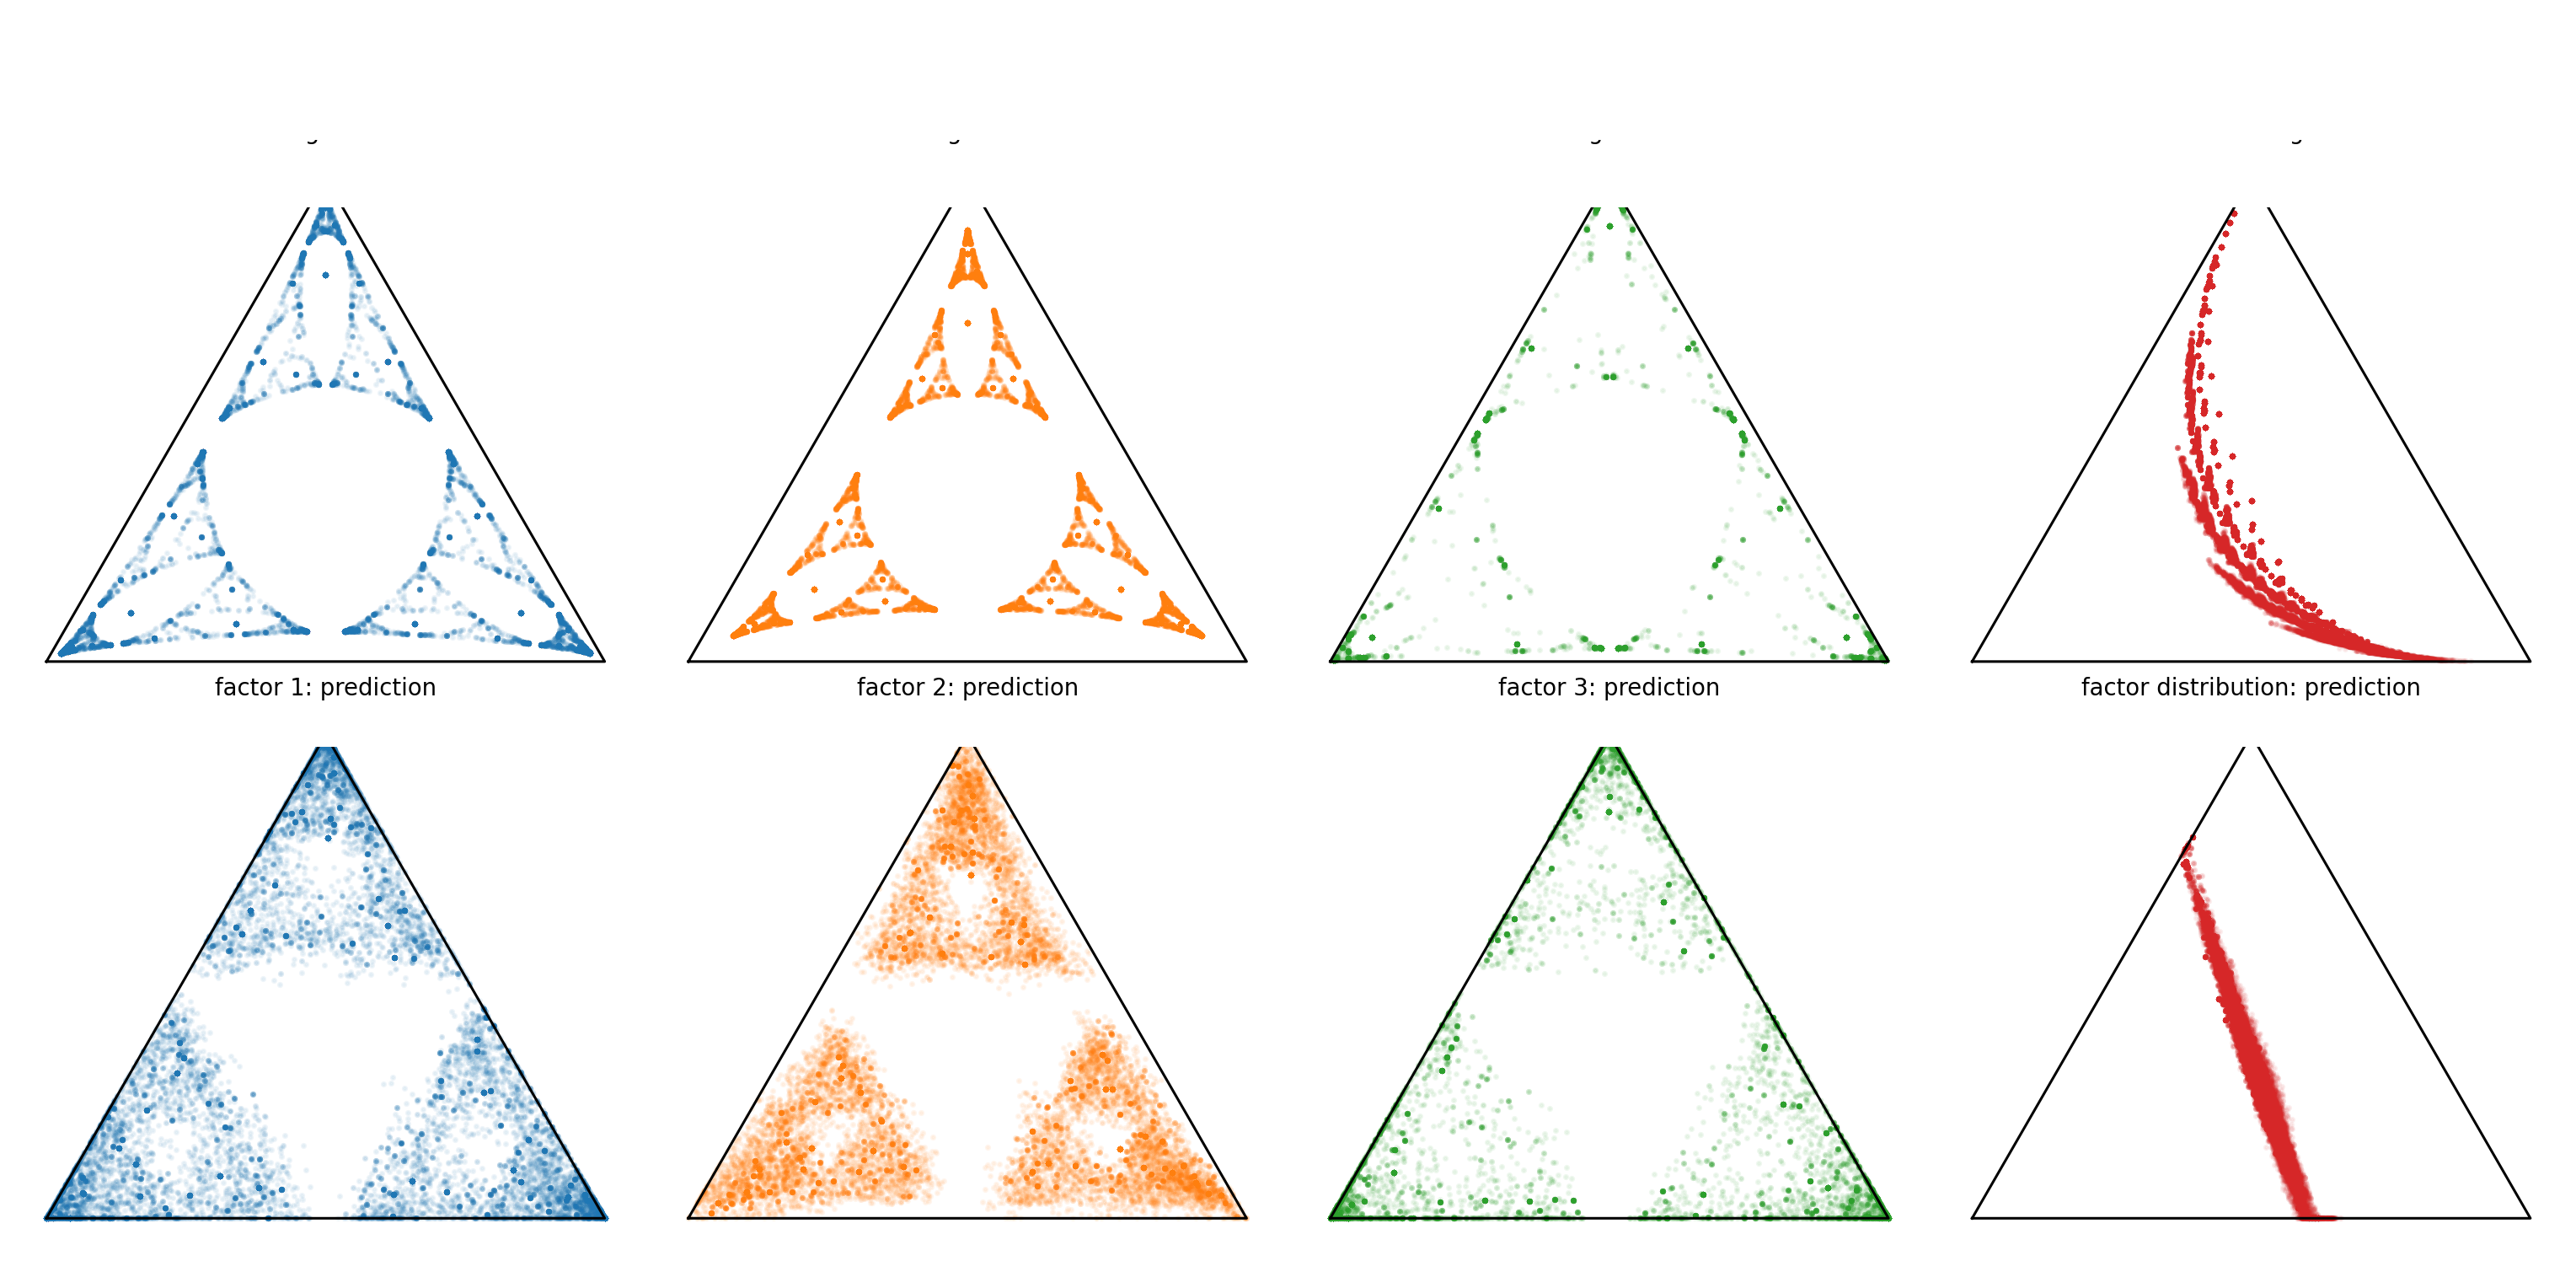
\includegraphics[width=\textwidth]{../artifacts/canonical_outputs/E2_side_by_side_simplex_trained_final_ln.png}
    \caption{Prediction and grouth truth plots of belief states of a common dataset.}
    \label{fig:e2_prob_trained}
\end{figure}

\begin{table}[ht]
    \centering
    \caption{KL-divergence between predicted belief state geometry based on least squares fit linear representation in residual stream and ground truth simplex belief state geometry}
    \label{tab:e1_kl}
    \begin{tabular}{lrr}
        \toprule
        Target & Trained & Control \\
        \midrule
        factor 1 & 0.1232 & 0.1533 \\
        factor 2 & 0.0156 & 0.0435 \\
        factor 3 & 0.0786 & 0.1120 \\
        factor distribution & 0.1065 & 0.1202 \\
        joint (8-simplex) & 1.2500 & 1.2489 \\
        \bottomrule
    \end{tabular}
\end{table}

The data in table \ref{tab:e1_kl} decisively shows that, contrary to my predictions, the belief state geometries of the factors have a linear representation and the belief state geometry of the entire process does not. Although the belief state geometry over the factors does not show an especially big change in KL-divegence compared to the control, figure \ref{fig:e2_prob_trained} demonstrates that it is signifcantly represented.

\subsection*{Using $\log$ Belief State Probabilites}

As mentioned in the introduction, there are mechanistic reasons for believing that the residual stream is more likely to represent the beliefs states using their log probabilites. Given the usual coodinates are, for example, $(p_1,p_2)$ we instead parameterise the simplex by $(\log(p_1/p_3),\log(p_2/p_3))$. These coordiantes are called additive log ratio coordinates which we refer to by ALR. We convert the ground truth belief state geometry into these coordinates and before performing the linear regression, and then convert back to probabilites before taking the the KL-divergence again.

\vspace{5mm}

This approach constsitently demonstrates superority compared with directly computing the probabilites, which supports that part of my hypothesis.
\begin{figure}[ht]
    \centering
    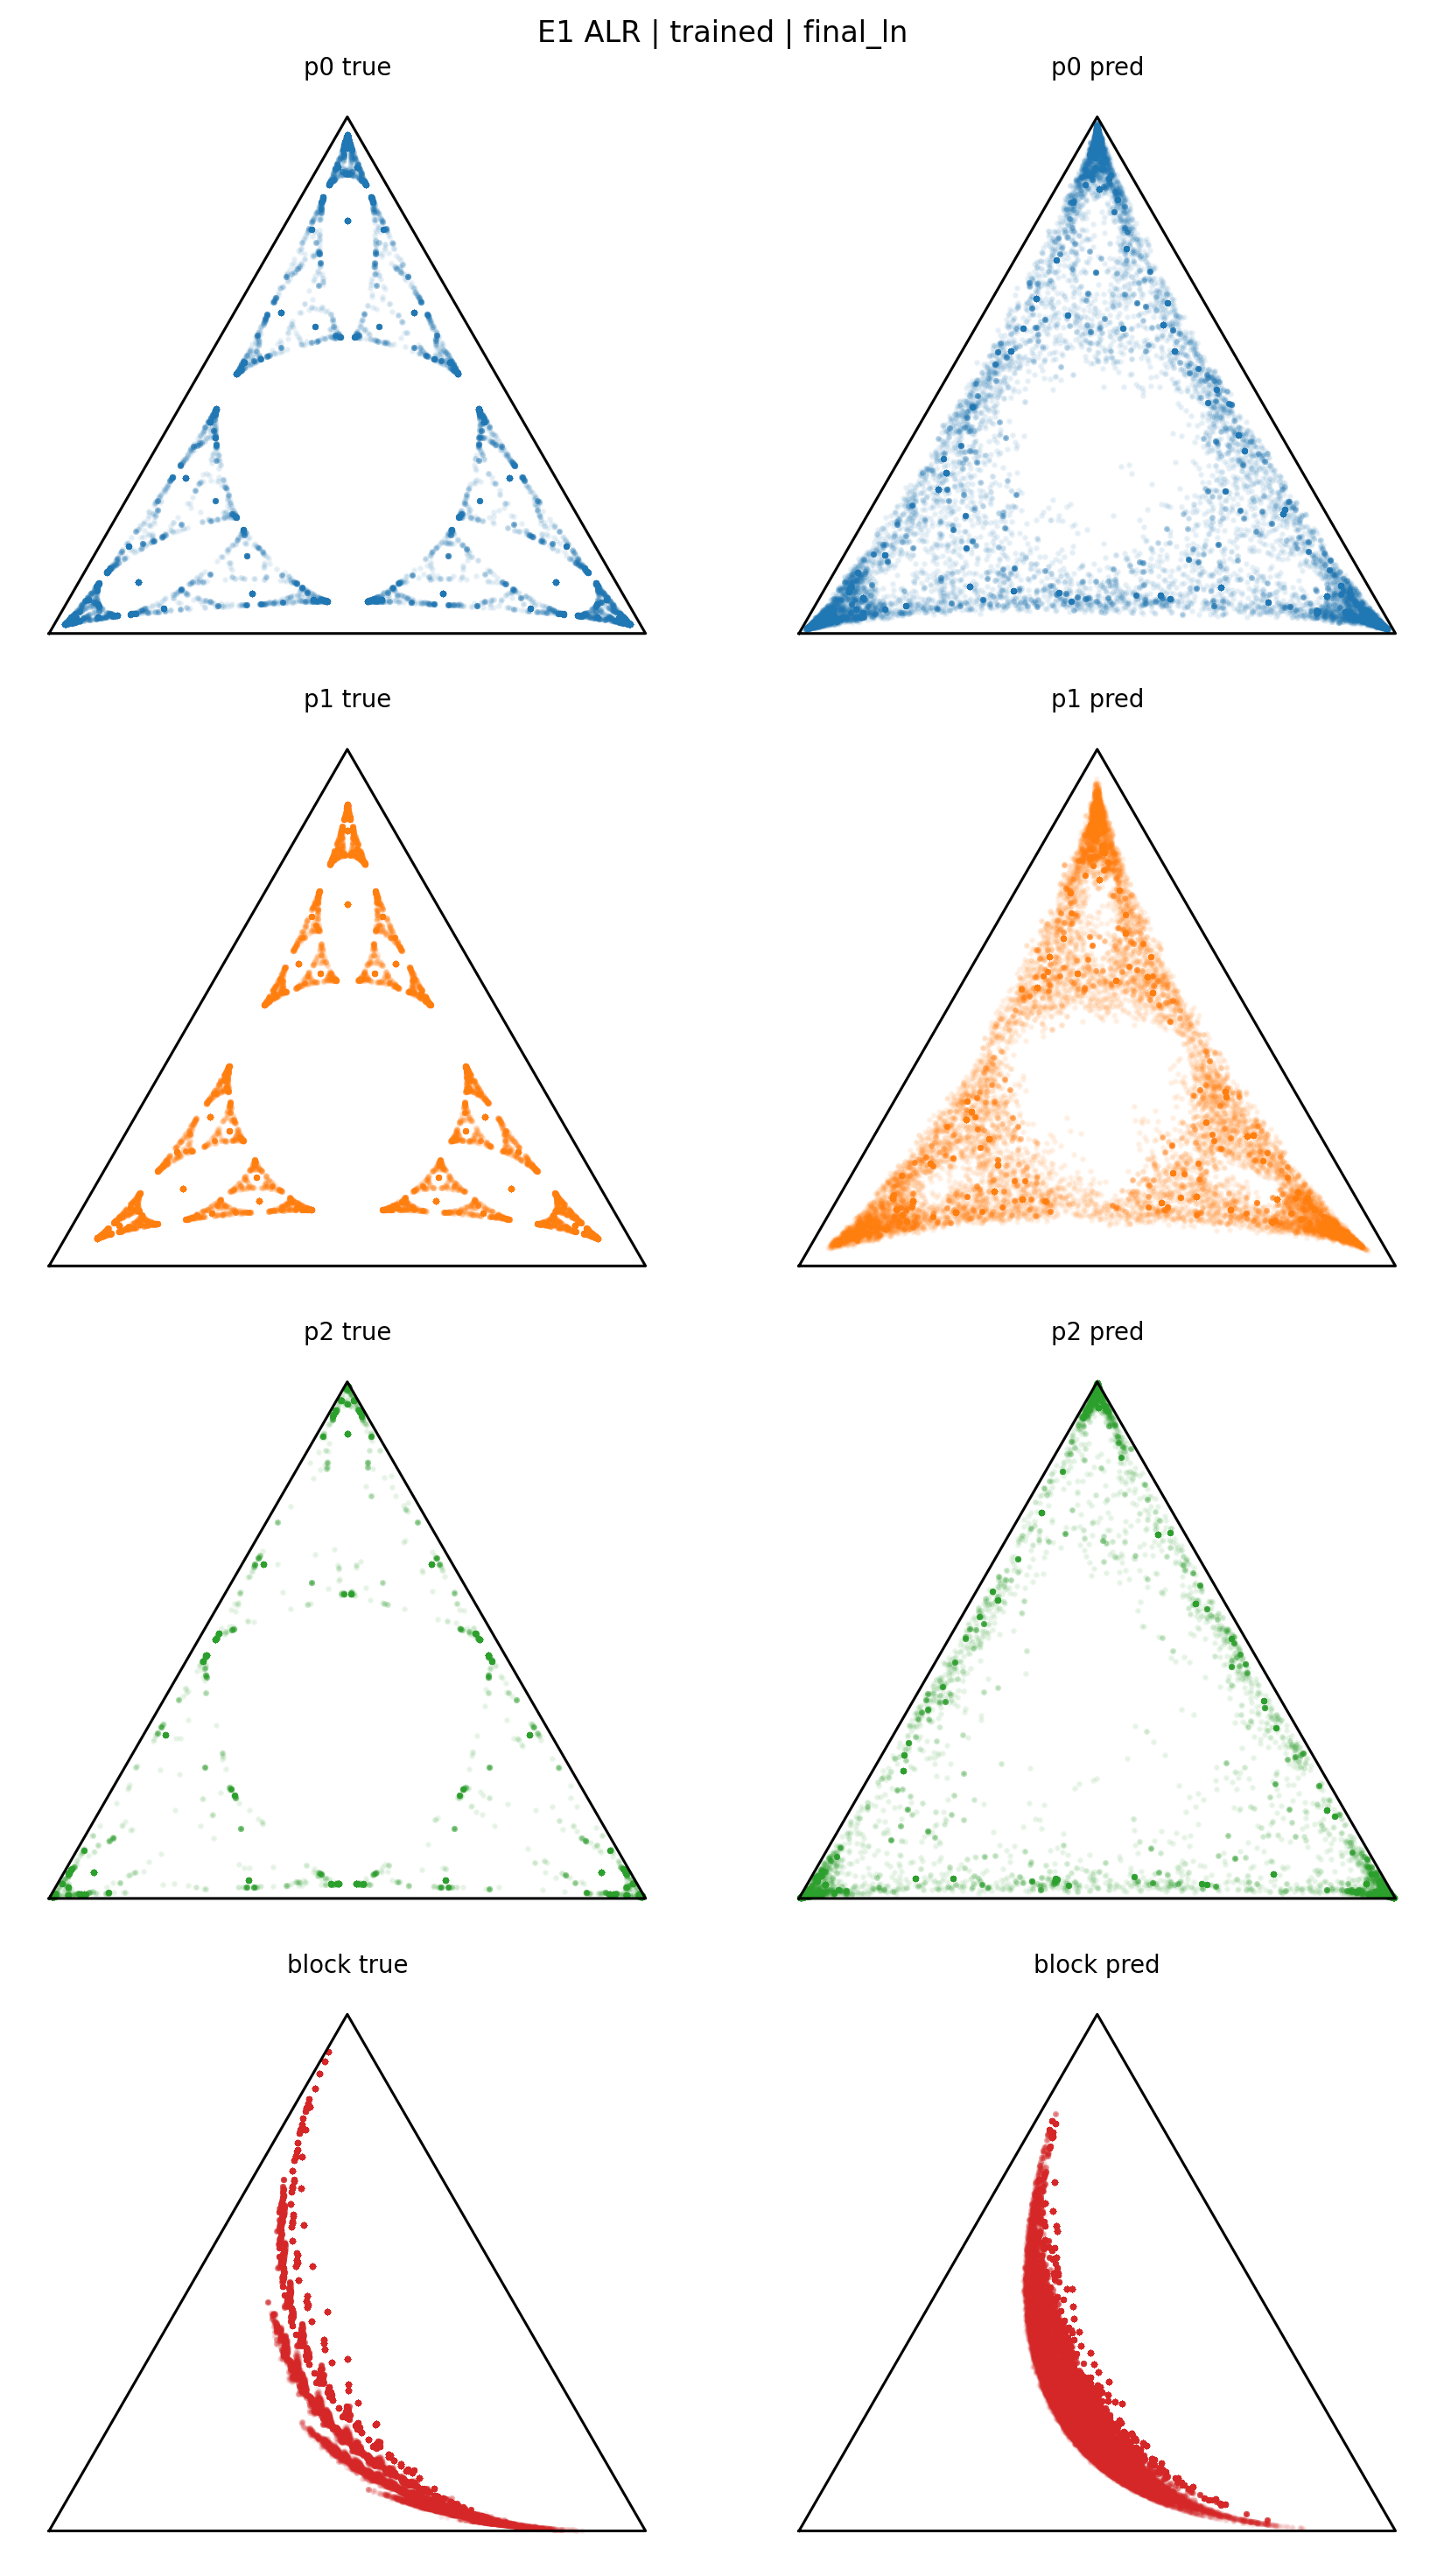
\includegraphics[width=\textwidth]{../artifacts/canonical_outputs/E1_side_by_side_simplex_trained_final_ln.png}
    \caption{Predictions created by least squares into ALR coordinates are then transformed to simplex coordinates before comparing using KL-divergence for a fair test.}
    \label{fig:e1_alr_trained}
\end{figure}

\begin{table}[ht]
    \centering
    \caption{The predictions created by using least squares into ALR coordinates are even more accurate to the ground truth when translated to simplex coordinates and compared using KL-divergence.}
    \label{tab:e2_kl}
    \begin{tabular}{lrr}
        \toprule
        Target & Trained & Control \\
        \midrule
        factor 1 & 0.0073 & 0.0484 \\
        factor 2 & 0.0037 & 0.0280 \\
        factor 3 & 0.0108 & 0.0569 \\
        factor distribution & 0.0865 & 0.1283 \\
        joint (8-simplex) & 1.6953 & 1.4928 \\
        \bottomrule
    \end{tabular}
\end{table}


\vspace{5mm}




\subsection*{Orthgonality in the Residual Stream}

In my hypothesis, the 4 representations occupy orthogonal subspaces in the residual stream. Conceptually, the factors are independent and a change in the reprsentation of one factor should not cause a change in the other facotor. That is, they should each be in the nullspaces of eachother's linear maps that we obtained via regression. I test this by calculating the principle angle between the rowspaces of each map.

\vspace{5mm}

Contrary to expectation, I find that while the representation of the belief state geometry across factors is close to orthogonal to the representations of the belief state geometries of the individual factors, they are not close to orthogonal to each other.

\begin{table}[ht]
    \centering
    \caption{Principle angles between row spaces of ALR maps. The representation of the belief state geometry over the factors is close to orthogonal to those of the individual factors, but the latter are aligned with eachother.}
    \label{tab:e3_within_angles_prob}
    \begin{tabular}{lrr}
        \toprule
        Pair & Trained & Control \\
        \midrule
        factor 1 vs factor 2 & 7.1060 & 9.0907 \\
        factor 1 vs factor 3 & 8.1205 & 11.4689 \\
        factor 2 vs factor 3 & 12.9379 & 18.2856 \\
        factor 1 vs factor distribution & 82.1118 & 82.5595 \\
        factor 2 vs factor distribution & 81.6707 & 82.3395 \\
        factor 3 vs factor distribution & 81.6074 & 82.0790 \\
        \bottomrule
    \end{tabular}
\end{table}

\vspace{5mm}

In retrospect it seems kind of obvious that because many Mess3 belief state geometries visually demonstrate so much geometric similarity to one another, it could be possible to store the state of multiple of them in a lower dimensional superposition. 

\vspace{3mm}

By doing linear regression between the ground truth simplex geometries we can find linear maps between them with close to $0$ kl-divergence. It appears that the model learns this shared structure and takes advantage of it to compress its representations. This was also alreaddy verified by the fact that the even in the control case with randomly initalised parameters, the regression found subspaces with a small principle angle between them.

\vspace{5mm}


suggest that this is a specific property of the mathematical simplicity of Mess3, and in general processes there would be substantailly less redundancy and different factors would be more likely to be represented orthogonally.

\begin{table}[ht]
    \centering
    \caption{Least squares fit to find a linear map between the ground truth 2-simplex data shows there are linear transforms wherein the belief state geometry of each factor are approximately the same, whereas the belief state geometry over factors is fundamentally distinct.}
    \label{tab:e4_alr_to_alr}
    \begin{tabular}{lrrrr}
        \toprule
        Source $\backslash$ Target & factor 1 & factor 2 & factor 3 & factor distribution \\
        \midrule
        factor 1 & 0.0000 & 0.0015 & 0.0029 & 0.1427 \\
        factor 2 & 0.0029 & 0.0000 & 0.0155 & 0.1452 \\
        factor 3 & 0.0016 & 0.0046 & 0.0000 & 0.1464 \\
        factor distribution & 0.6011 & 0.4116 & 0.7596 & 0.0000 \\
        \bottomrule
    \end{tabular}
\end{table}





\subsection*{Intervening to Supress a Factor}

As mentioned in the introduction, the independent factors in the data-generating process bear some resemblance to the empirically observed phenomena of personas in LLMs. The belief state geometry we have demonstrated in this work is therefore the best case because, by analogy, the probability of being in a given persona is decoupled from the beliefs about what each persona would do next. We consider how our findings could be used to supress a broadly misaligned persona in this analogy \cite{betley2025emergentmisalignment}.

\vspace{5mm}

Suppose that the third Mess3 factor is undesirable. In ALR coodinates we can reduce the probability $p_3$ of belief of being in this factor:

$$(\log(p_1/p_3),\log(p_2/p_3))\mapsto (\log(p_1/p_3)+\delta,\log(p_2/p_3)+\delta)=(\log(p_1/(p_3\exp(-\delta))),\log(p_2/\exp(-\delta))).$$

In order to induce this effect, we choose a steering vector $s$ in the null space of all three linear maps into into the individual factors so that it doesn't affect the model's reprsentations of their belief state geometries. For a vector in the residual stream $r$, we define $\delta_1,\delta_2$ so that in the ALR coordinates:

$$L(r+s)=(L_0(r)_1+\delta_1,L(r)_2+\delta_2),$$

and use the Adam optmiser to find $s$ maximising:

$$\min(\delta_1,\delta_2)-\lambda(\delta_1-\delta_2)^2+\beta \sum_{i=1}^3||L_i(s)||^2$$

for some fixed choice of parameters $\lambda,\beta$. That is, we find the steer that drops the probability of one factor as much as possible while penalising it not retaining the ratio between the other factors or leaving the nullspace of any of the maps (and therefore affecting the beliefs over the hidden states).

\vspace{5mm}

In order to test this approach, We generate three datasets of sequences, each including only two of the three data generating processes. We test all three steering vectors on all three datasets, hypothesising that the steering vector corresponding to loading the probability of a given factor will perform best on the dataset excluding data generated by that factor.

\vspace{5mm}

\begin{table}[ht]
    \centering
    \caption{The cross-entropy losses obtained from using the different steering vectors on the different datasets do not show an effect.}
    \label{tab:e6_steering_cross_eval_loss}
    \begin{tabular}{lrrr}
        \toprule
        Dataset & $p_1\downarrow$ steer & $p_2\downarrow$ steer& $p_3\downarrow$ steer \\
        \midrule
        Factor 1 omitted & 0.99183965 & 0.98798378 & 0.98698572 \\
        Factor 2 omittedd & 1.10878269 & 1.10895218 & 1.10783441 \\
        Factor 3 omitted & 0.74529040 & 0.74673929 & 0.74574044 \\
        \bottomrule
    \end{tabular}
\end{table}

As shown in the table, we find a null result. We can likely attribute this to the steering method being too heavy-handed and damaging the belief state geometry or other representations to an extent that completely noises the results.


\vspace{5mm}

Time permitting, I would devise a more targeted method for this steering.
\subsection*{Further Directions}

In this section I will list some of my ideas of what I would try next (I am very interested in this research if you can't tell from my writing).

\vspace{3mm}

The overall research agenda in this area would be to establish a general description of the inductive biases that transformers have in choosing geometry to represent the true belief state geometries of the kind of `cascading' hidden markov models we describe here.


\vspace{3mm}
To have a serious theory of impact, it should at least make some predictions about large langauge models that are falsifiable.

\begin{itemize}
    \item Use more mathematically distinct factors of the data-generating process than the Mess3 procesess in this work to see whether repesentations of factors form in orthogonal subspaces.
    \item As a theoretical exercise, try to describe (an) attention head(s) that would actually do the computation of the belief state geometry. Would this algorithm scale arbitrarily with the size of the context window? Test this prediction.
    \item Stack more layers of hidden Markov process, to create a data-generating process with more non-ergodic depth. That is, the sequence globally belongs to some factor, but there is a directed graph between subfactors that the state can move between to generate subsequences. Again the question is what level of structure is represented in the residual stream?
\end{itemize}


\bibliographystyle{unsrtnat}
\bibliography{references}

\end{document}
